\documentclass[11pt]{article}
\usepackage[utf8]{inputenc}	% Para caracteres en español
\usepackage{amsmath,amsthm,amsfonts,amssymb,amscd}
\usepackage{multirow,booktabs}
\usepackage[table]{xcolor}
\usepackage{fullpage}
\usepackage{lastpage}
\usepackage{enumitem}
\usepackage{fancyhdr}
\usepackage{mathrsfs}
\usepackage{wrapfig}
\usepackage{setspace}
\usepackage{calc}
\usepackage{multicol}
\usepackage{cancel}
\usepackage{float}
\usepackage{physics}
\usepackage[retainorgcmds]{IEEEtrantools}
\usepackage[margin=1cm]{geometry}
\usepackage{amsmath}
\newlength{\tabcont}
\setlength{\headheight}{14pt}
\setlength{\parindent}{0.0in}
\setlength{\parskip}{0.05in}
\usepackage{empheq}
\usepackage{framed}
\usepackage[most]{tcolorbox}
\usepackage{xcolor}
\usepackage[version=3]{mhchem}
\usepackage[english]{babel}
\usepackage[utf8]{inputenc}
\usepackage{graphicx}
\usepackage[colorinlistoftodos]{todonotes}
\usepackage{mdframed}

\colorlet{shadecolor}{orange!15}
\parindent 0in
\parskip 12pt
\geometry{margin=1in, headsep=0.45in}
\theoremstyle{definition}
\newtheorem{defn}{Definition}
\newtheorem{reg}{Rule}
\newtheorem{exer}{Exercise}
\newtheorem{note}{Note}
\begin{document}
\setcounter{section}{2}
%\setcounter{subsection}{}
\title{Problem Set 10}

%==============================================================
%\thispagestyle{empty}
\pagestyle{fancy}
\fancyhf{}
\rhead{Physics 180}
\chead{Problem Set 10}
\lhead{Olyn D. Desabelle}
\rfoot{Page \thepage}

\begin{center}
{\LARGE \bf Problem Set 10}\\
%{\large Physics 180}\\
%Olyn D. Desabelle
\end{center}

%==============================================================
\begin{figure}[H]
    \centering
    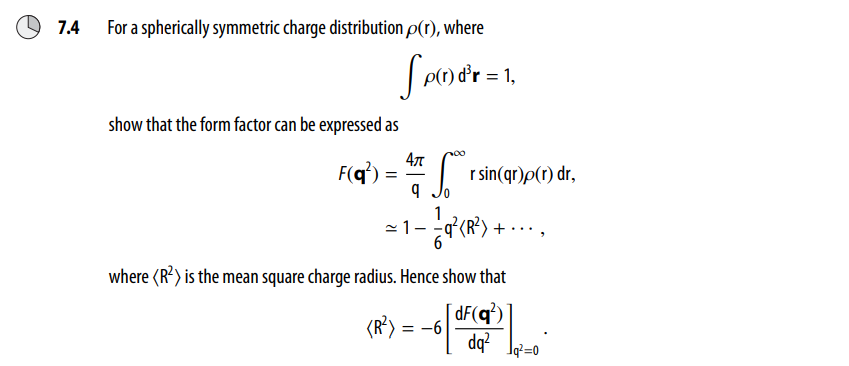
\includegraphics[scale = 0.5]{7.4.png}
\end{figure}

We begin with the definition of the form factor as:

\begin{align}
    F (\mathbf{q^2}) = \int \rho(\mathbf{r}) e^{i\mathbf{q}\cdot\mathbf{r}}\; d^3\mathbf{r}
\end{align}

evalutating in spherical coordinates, noting that the dot product $\mathbf{q}\cdot\mathbf{r} = qr\cos\theta$ , this becomes:

\begin{align}
    F (\mathbf{q^2}) &= \int_{\theta=0}^{\theta=\pi}
    \int_{\phi=0}^{\phi=2\pi}
    \int_{r=0}^{r=\infty}  \rho(\mathbf{r}) e^{i\mathbf{q}\cdot\mathbf{r}}\; r^2 \sin\theta\; dr\; d\phi\; d\theta\\
    &= 
    \int_{\phi=0}^{\phi=2\pi}
    d\phi
    \int_{\theta=0}^{\theta=\pi}
    \int_{r=0}^{r=\infty}  \rho(\mathbf{r}) e^{iqr\cos\theta}\; r^2 \; dr\;\sin\theta \; d\theta\\
    &= 2\pi \int_{r=0}^{r=\infty} \left[\int_{\theta=0}^{\theta=\pi} e^{iqr\cos\theta}\sin\theta \; d\theta \right] r^2 \rho(\mathbf{r}) \; dr
\end{align}

rewriting $\sin\theta\; d\theta = d(\cos\theta)$, we get:

\begin{align}
    F (\mathbf{q^2}) &= 2\pi \int_{r=0}^{r=\infty} \left[\int_{\theta=0}^{\theta=\pi} e^{iqr\cos\theta} d(\cos\theta) \right] r^2 \rho(\mathbf{r}) \; dr\\
    &= 2\pi \int_{r=0}^{r=\infty} \left[\int_{\cos\theta=-1}^{\cos\theta=1} e^{iqr\cos\theta} d(\cos\theta) \right] r^2 \rho(\mathbf{r}) \; dr\\
    &= 2\pi \int_{r=0}^{r=\infty} 
    \left[ \frac{-i\left(e^{iqr}-e^{-iqr}\right)}{qr} \right] r^2 \rho(\mathbf{r}) \; dr\\
    &= 2\pi \int_{r=0}^{r=\infty} 
    \left[ \frac{\left(e^{iqr}-e^{-iqr}\right)}{iq} \right] r \rho(r) \; dr\\
\end{align}

noting that $\sin(x) = \frac{e^{ix}-e^{-ix}}{2i}$, we may rewrite this as:

\begin{align}
    F (\mathbf{q^2}) &= 2\pi \int_{r=0}^{r=\infty} 
    \left[ \frac{\left(e^{iqr}-e^{-iqr}\right)}{iq} \right] \left(\frac{2}{2}\right) r \rho(r)\; dr\\
\end{align}

\begin{equation}
\boxed{
    F (\mathbf{q^2}) = \frac{4\pi}{q} \int_{r=0}^{r=\infty} 
    r\sin(qr)   \rho(r) \; dr\\
}
\end{equation}

expanding the $\sin(qr)$ term as its Taylor expansion $\sin(x) = x - \frac{x^3}{3!} + \frac{x^5}{5!} - \frac{x^7}{7!} + \dots$ we have:

\begin{align}
    F (\mathbf{q^2}) 
    &=  \frac{4\pi}{q} \int_{r=0}^{r=\infty} 
    \sin(qr)  r \rho(r)  \; dr\\
    &= \frac{4\pi}{q} \int_{r=0}^{r=\infty} 
    r \rho(r) \sin(qr) \; dr\\
    &= \frac{4\pi}{q} \int_{r=0}^{r=\infty} 
    r \rho(r) \left[qr - \frac{(qr)^3}{3!} + \dots \right] \; dr\\
    &= \frac{4\pi}{q} \int_{r=0}^{r=\infty} 
    r \rho(r) \left[qr - \frac{(qr)^3}{6} + \dots \right] \; dr
\end{align}

we note the given condition for a given spherically symmetric charge distribution $\rho(r)$ such that:

\begin{align}
    \int \rho(r) d^3\mathbf{r} = 1
\end{align}

performing the integral in spherical coordinates gives:

\begin{align}
    \int_{\phi=0}^{\phi=2\pi}\int_{\theta=0}^{\theta=\pi}\int_{r=0}^{r=\infty} \rho(r) r^2 \sin\theta\; dr\; d\phi\; d\theta  &= 1\\
    4\pi \int_{r=0}^{r=\infty}  r^2\; \rho(r) dr &= 1
\end{align}

thus the form factor becomes:

\begin{align}
    F (\mathbf{q^2})  &= 
    4\pi \int_{r=0}^{r=\infty} 
    r^2 \rho(r) \; dr  - \frac{1}{6}q^2 \left(4\pi \int_{r=0}^{r=\infty} r^4 \; dr \right)  + \dots\\
    &=
    1 - \frac{1}{6}q^2 \left(4\pi \int_{r=0}^{r=\infty} r^4 \; dr \right)  + \dots\\
\end{align}

with the mean square charge radius $\expval{R^2} = 4\pi \int_{r=0}^{r=\infty} r^4 \; dr $, then this becomes:

\begin{equation}
\boxed{
    F (\mathbf{q^2}) \approx 1-\frac{1}{6}q^2 \expval{R^2}
}
\end{equation}

differentiating this with respect to $q^2$, we have:

\begin{align}
    \frac{dF (\mathbf{q}^2)}{dq^2} &= \frac{d}{dq^2} \left[1-\frac{1}{6}q^2 \expval{R^2}\right]\\
    \frac{dF (\mathbf{q}^2)}{dq^2} &= -\frac{1}{6} \expval{R^2}\\
    \expval{R^2} &= -6 \left[\frac{dF (\mathbf{q}^2)}{dq^2}\right]
\end{align}

since for higher values of $\mathbf{q}^2$, the elastic scattering cross section tends to zero ($F(\mathbf{q}^2\to\infty)=0$), then:

\begin{equation}
\boxed{
    \expval{R^2} = -6 \left[\frac{dF (\mathbf{q}^2)}{dq^2}\right]_{q^2=0}
}
\end{equation}
\newpage
%==============================================================
\begin{figure}[H]
    \centering
    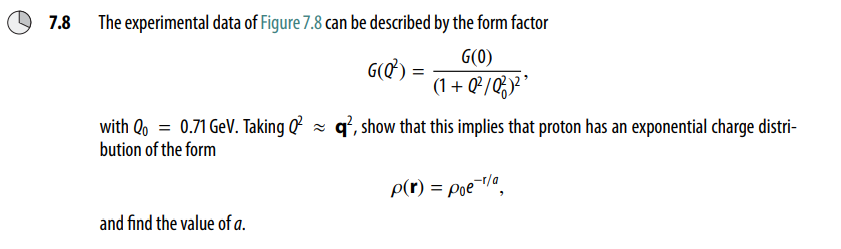
\includegraphics[scale = 0.5]{7.8.png}
\end{figure}

The form factor in spherical coordinates is given by:

\begin{align}
    G(q^2) &= \int \rho(\mathbf{r}) e^{i\mathbf{q}\cdot\mathbf{r}}\; d^3\mathbf{r}\\
    &= \int_{\theta=0}^{\theta=\pi}
    \int_{\phi=0}^{\phi=2\pi}
    \int_{r=0}^{r=\infty}  \rho(\mathbf{r})e^{i\mathbf{q}\cdot\mathbf{r}} \; r^2 \sin\theta\; dr\; d\phi\; d\theta\\
\end{align}

this is similar to the earlier problem, where we get:

\begin{align}
    G(q^2) &= \frac{4\pi}{q} \int_{r=0}^{r=\infty} 
    r\sin(qr)   \rho(r) \; dr
\end{align}

with the given charge distribution $\rho(\mathbf{r}) = \rho_0 e^{-r/a}$, this becomes:

\begin{align}
    G(q^2) &= \frac{4\pi\rho_0}{q} \int_{r=0}^{r=\infty} 
    r\sin(qr)  e^{-r/a}\; dr
\end{align}

rewriting the sine term in its exponential form, we have:

\begin{align}
    G(q^2) &= \frac{4\pi\rho_0}{q} \int_{r=0}^{r=\infty} 
    r \left[\frac{e^{iqr}-e^{-iqr}}{2i}\right] e^{-r/a}\; dr\\
    &= \frac{2\pi\rho_0}{iq} \int_{r=0}^{r=\infty} 
    r e^{-r/a+iqr} \; dr -  \frac{2\pi\rho_0}{iq} \int_{r=0}^{r=\infty} 
    re^{-r/a-iqr}\; dr\\
\end{align}

with $u=r$ and $v$ as the exponential term, integration by parts $\int udv = uv-\int vdu$ gives:

\begin{align}
    G(q^2) &= \frac{2\pi\rho_0}{iq} 
    \left(
       \frac{1}{[(1/a)-iq]^2} - \frac{1}{[(1/a)+iq]^2}
    \right)\\
    G(q^2) &= \frac{2\pi\rho_0}{iq} 
    \left( i\frac{4(q/a)}{(1/a)^4+q^4+2(1/a)^2q^2}\right)\\
    %G(q^2) &= \frac{8\pi\rho_0}{a}  \left(\frac{1}{((1/a)^2+q^2)^2}\right)\\ 
    G(q^2) &= 8\pi\rho_0 a^3 \left(\frac{1}{(1+a^2q^2)^2}\right) 
\end{align}

we note that at $q^2=0$, we have:

\begin{align}
    G(0) &= 8\pi\rho_0 a^3 
\end{align}

we may rewrite the form factor as: 

\begin{align}
    G(q^2) &=  \frac{G(0)}{(1+a^2q^2)^2}
\end{align}

comparing this to the given form factor, we see that:

\begin{align}
    &G(q^2) =  \frac{G(0)}{(1+a^2q^2)^2}
    \;\;\;\;\;\;\;\;\;\;
    G(Q^2) = \frac{G(0)}{(1+Q^2/Q_0^2)^2}\\
    &\implies q^2=Q^2,\;\;\; a^2 = 1/Q_0^2  
\end{align}

from this we may find the value for $a$ with the given $Q_0 = 0.71\; \text{GeV}$:

\begin{align}
    a = \sqrt{\frac{1}{(0.71\; \text{GeV})^2}}
\end{align}

\begin{equation}
\boxed{
    a = 1.41\;\text{GeV}
}
\end{equation}
%==============================================================
\end{document}